\documentclass[conference]{IEEEtran}
\IEEEoverridecommandlockouts
\usepackage{iftex}
\ifPDFTeX
  \usepackage[utf8]{inputenc}
\fi
% T1 Times under pdfLaTeX (Overleaf) and XeTeX (Tectonic) alike, as IEEEtran expects
\usepackage[T1]{fontenc}
\usepackage{cite}
\usepackage{amsmath,amssymb}
\usepackage{graphicx}
\usepackage{booktabs}
\usepackage{xcolor}
\usepackage{url}
\usepackage{tikz}
\usetikzlibrary{positioning,fit,arrows.meta,shapes.geometric,calc}
\usepackage[hidelinks]{hyperref}

% Results, generated by eval/make_macros.py from eval/results/*; it also defines the switches
% \ifrecheck and \ifmentoring, which are true only when those experiments are complete.
% Generated by eval/make_macros.py — do not edit by hand
\newcommand{\ResAudioCpGemAudioClean}{21.7}
\newcommand{\ResAudioCpGemAudioFive}{23.1}
\newcommand{\ResAudioCpGemAudioZero}{54.6}
\newcommand{\ResAudioCpSbEnhClean}{43.8}
\newcommand{\ResAudioCpSbEnhFive}{44.3}
\newcommand{\ResAudioCpSbEnhZero}{76.1}
\newcommand{\ResAudioCpSbRawClean}{30.5}
\newcommand{\ResAudioCpSbRawFive}{52.6}
\newcommand{\ResAudioCpSbRawZero}{65.1}
\newcommand{\ResAudioCpTextClean}{42.3}
\newcommand{\ResAudioCpTextFive}{29.2}
\newcommand{\ResAudioCpTextZero}{58.8}
\newcommand{\ResAudioDerSbEnhClean}{26.9}
\newcommand{\ResAudioDerSbEnhFive}{19.3}
\newcommand{\ResAudioDerSbEnhZero}{25.7}
\newcommand{\ResAudioDerSbRawClean}{25.1}
\newcommand{\ResAudioDerSbRawFive}{28.7}
\newcommand{\ResAudioDerSbRawZero}{26.8}
\newcommand{\ResAudioWerGemEnhClean}{2.9}
\newcommand{\ResAudioWerGemEnhFive}{19.3}
\newcommand{\ResAudioWerGemEnhZero}{63.6}
\newcommand{\ResAudioWerGemRawClean}{1.7}
\newcommand{\ResAudioWerGemRawFive}{14.7}
\newcommand{\ResAudioWerGemRawZero}{44.8}
\newcommand{\ResAudioWerGroqEnhClean}{2.1}
\newcommand{\ResAudioWerGroqEnhFive}{21.2}
\newcommand{\ResAudioWerGroqEnhZero}{63.9}
\newcommand{\ResAudioWerGroqRawClean}{2.0}
\newcommand{\ResAudioWerGroqRawFive}{8.9}
\newcommand{\ResAudioWerGroqRawZero}{32.1}
\newcommand{\ResCascadeAfter}{5.8\%}
\newcommand{\ResCascadeBefore}{6.7\%}
\newcommand{\ResCascadeEscalated}{1}
\newcommand{\ResCascadeNotes}{37}
\newcommand{\ResCascadeOverGateAfter}{0}
\newcommand{\ResCascadeSwitched}{1}
\newcommand{\ResGroundGemCited}{95.4\%}
\newcommand{\ResGroundGemNotes}{38}
\newcommand{\ResGroundGemOverGate}{1}
\newcommand{\ResGroundGemPartial}{9.4\%}
\newcommand{\ResGroundGemSentences}{18.2}
\newcommand{\ResGroundGemSupported}{83.4\%}
\newcommand{\ResGroundGemUnsupported}{7.2\%}
\newcommand{\ResGroundGroqCited}{97.2\%}
\newcommand{\ResGroundGroqNotes}{39}
\newcommand{\ResGroundGroqOverGate}{4}
\newcommand{\ResGroundGroqPartial}{16.2\%}
\newcommand{\ResGroundGroqSentences}{16.7}
\newcommand{\ResGroundGroqSupported}{76.9\%}
\newcommand{\ResGroundGroqUnsupported}{6.9\%}
\newcommand{\ResInjControlN}{129}
\newcommand{\ResInjFaPct}{9\%}
\newcommand{\ResInjGemFa}{7\%}
\newcommand{\ResInjGemFab}{100\%}
\newcommand{\ResInjGemFabN}{20}
\newcommand{\ResInjGemNeg}{100\%}
\newcommand{\ResInjGemNegN}{12}
\newcommand{\ResInjGemNum}{95\%}
\newcommand{\ResInjGemNumN}{20}
\newcommand{\ResInjGemRecall}{98\%}
\newcommand{\ResInjGemVerifier}{Google Gemini (gemini-3.5-flash)}
\newcommand{\ResInjGroqFa}{12\%}
\newcommand{\ResInjGroqFab}{100\%}
\newcommand{\ResInjGroqFabN}{23}
\newcommand{\ResInjGroqNeg}{100\%}
\newcommand{\ResInjGroqNegN}{13}
\newcommand{\ResInjGroqNum}{95\%}
\newcommand{\ResInjGroqNumN}{21}
\newcommand{\ResInjGroqRecall}{98\%}
\newcommand{\ResInjGroqVerifier}{Google Gemini (gemini-3.5-flash)}
\newcommand{\ResInjPlantedN}{109}
\newcommand{\ResInjRecallPct}{98\%}
\newcommand{\ResLatGemDiar}{46.8}
\newcommand{\ResLatSbDiar}{13.0}
\newcommand{\ResLatSbEnh}{74.1}
\newcommand{\ResLatSttGem}{41.3}
\newcommand{\ResLatSttGroq}{12.8}
\newcommand{\ResLatTextDiar}{62.2}
\newcommand{\ResNoteGemBert}{48.0}
\newcommand{\ResNoteGemN}{40}
\newcommand{\ResNoteGemRougeL}{42.5}
\newcommand{\ResNoteGemRougeOne}{45.4}
\newcommand{\ResNoteGemRougeTwo}{16.9}
\newcommand{\ResNoteGemSecs}{39}
\newcommand{\ResNoteGroqBert}{42.7}
\newcommand{\ResNoteGroqN}{40}
\newcommand{\ResNoteGroqRougeL}{41.7}
\newcommand{\ResNoteGroqRougeOne}{45.9}
\newcommand{\ResNoteGroqRougeTwo}{14.2}
\newcommand{\ResNoteGroqSecs}{50}
\newcommand{\ResRoleCombined}{97.5\%}
\newcommand{\ResRoleCombinedCorrect}{39}
\newcommand{\ResRoleHardCombined}{1}
\newcommand{\ResRoleHardLlm}{1}
\newcommand{\ResRoleHardN}{2}
\newcommand{\ResRoleHardStats}{1}
\newcommand{\ResRoleLlm}{92.5\%}
\newcommand{\ResRoleLlmCorrect}{37}
\newcommand{\ResRoleN}{40}
\newcommand{\ResRoleStats}{95.0\%}
\newcommand{\ResRoleStatsCorrect}{38}
\newcommand{\ResRouterMixedFixedCalls}{1.13}
\newcommand{\ResRouterMixedFixedFailed}{0.147}
\newcommand{\ResRouterMixedFixedJain}{0.64}
\newcommand{\ResRouterMixedFixedMean}{3.68}
\newcommand{\ResRouterMixedFixedPninetyfive}{31.5}
\newcommand{\ResRouterMixedFixedSuccess}{98.14\%}
\newcommand{\ResRouterMixedLkgpCalls}{1.10}
\newcommand{\ResRouterMixedLkgpFailed}{0.097}
\newcommand{\ResRouterMixedLkgpJain}{0.49}
\newcommand{\ResRouterMixedLkgpMean}{2.75}
\newcommand{\ResRouterMixedLkgpPninetyfive}{9.1}
\newcommand{\ResRouterMixedLkgpSuccess}{100.00\%}
\newcommand{\ResRouterMixedNomemoryCalls}{1.50}
\newcommand{\ResRouterMixedNomemoryFailed}{0.497}
\newcommand{\ResRouterMixedNomemoryJain}{0.49}
\newcommand{\ResRouterMixedNomemoryMean}{3.79}
\newcommand{\ResRouterMixedNomemoryPninetyfive}{31.8}
\newcommand{\ResRouterMixedNomemorySuccess}{99.93\%}
\newcommand{\ResRouterMixedPriorityCalls}{1.26}
\newcommand{\ResRouterMixedPriorityFailed}{0.258}
\newcommand{\ResRouterMixedPriorityJain}{0.49}
\newcommand{\ResRouterMixedPriorityMean}{3.88}
\newcommand{\ResRouterMixedPriorityPninetyfive}{31.7}
\newcommand{\ResRouterMixedPrioritySuccess}{99.86\%}
\newcommand{\ResRouterMixedRoundrobinCalls}{1.09}
\newcommand{\ResRouterMixedRoundrobinFailed}{0.092}
\newcommand{\ResRouterMixedRoundrobinJain}{0.66}
\newcommand{\ResRouterMixedRoundrobinMean}{3.48}
\newcommand{\ResRouterMixedRoundrobinPninetyfive}{31.4}
\newcommand{\ResRouterMixedRoundrobinSuccess}{100.00\%}
\newcommand{\ResRouterOutageFixedCalls}{1.09}
\newcommand{\ResRouterOutageFixedFailed}{0.087}
\newcommand{\ResRouterOutageFixedJain}{0.73}
\newcommand{\ResRouterOutageFixedMean}{1.35}
\newcommand{\ResRouterOutageFixedPninetyfive}{2.4}
\newcommand{\ResRouterOutageFixedSuccess}{99.89\%}
\newcommand{\ResRouterOutageLkgpCalls}{1.04}
\newcommand{\ResRouterOutageLkgpFailed}{0.040}
\newcommand{\ResRouterOutageLkgpJain}{0.87}
\newcommand{\ResRouterOutageLkgpMean}{1.27}
\newcommand{\ResRouterOutageLkgpPninetyfive}{2.4}
\newcommand{\ResRouterOutageLkgpSuccess}{99.93\%}
\newcommand{\ResRouterOutageNomemoryCalls}{1.29}
\newcommand{\ResRouterOutageNomemoryFailed}{0.291}
\newcommand{\ResRouterOutageNomemoryJain}{0.68}
\newcommand{\ResRouterOutageNomemoryMean}{1.47}
\newcommand{\ResRouterOutageNomemoryPninetyfive}{2.4}
\newcommand{\ResRouterOutageNomemorySuccess}{99.97\%}
\newcommand{\ResRouterOutagePriorityCalls}{1.06}
\newcommand{\ResRouterOutagePriorityFailed}{0.062}
\newcommand{\ResRouterOutagePriorityJain}{0.77}
\newcommand{\ResRouterOutagePriorityMean}{1.31}
\newcommand{\ResRouterOutagePriorityPninetyfive}{2.3}
\newcommand{\ResRouterOutagePrioritySuccess}{99.97\%}
\newcommand{\ResRouterOutageRoundrobinCalls}{1.06}
\newcommand{\ResRouterOutageRoundrobinFailed}{0.058}
\newcommand{\ResRouterOutageRoundrobinJain}{0.83}
\newcommand{\ResRouterOutageRoundrobinMean}{1.41}
\newcommand{\ResRouterOutageRoundrobinPninetyfive}{2.7}
\newcommand{\ResRouterOutageRoundrobinSuccess}{99.93\%}
\newcommand{\ResRouterQuotaFixedCalls}{1.10}
\newcommand{\ResRouterQuotaFixedFailed}{0.098}
\newcommand{\ResRouterQuotaFixedJain}{0.79}
\newcommand{\ResRouterQuotaFixedMean}{1.29}
\newcommand{\ResRouterQuotaFixedPninetyfive}{2.3}
\newcommand{\ResRouterQuotaFixedSuccess}{100.00\%}
\newcommand{\ResRouterQuotaLkgpCalls}{1.03}
\newcommand{\ResRouterQuotaLkgpFailed}{0.033}
\newcommand{\ResRouterQuotaLkgpJain}{0.54}
\newcommand{\ResRouterQuotaLkgpMean}{1.05}
\newcommand{\ResRouterQuotaLkgpPninetyfive}{1.9}
\newcommand{\ResRouterQuotaLkgpSuccess}{99.97\%}
\newcommand{\ResRouterQuotaNomemoryCalls}{1.48}
\newcommand{\ResRouterQuotaNomemoryFailed}{0.476}
\newcommand{\ResRouterQuotaNomemoryJain}{0.63}
\newcommand{\ResRouterQuotaNomemoryMean}{1.46}
\newcommand{\ResRouterQuotaNomemoryPninetyfive}{2.4}
\newcommand{\ResRouterQuotaNomemorySuccess}{99.97\%}
\newcommand{\ResRouterQuotaPriorityCalls}{1.23}
\newcommand{\ResRouterQuotaPriorityFailed}{0.227}
\newcommand{\ResRouterQuotaPriorityJain}{0.65}
\newcommand{\ResRouterQuotaPriorityMean}{1.40}
\newcommand{\ResRouterQuotaPriorityPninetyfive}{2.4}
\newcommand{\ResRouterQuotaPrioritySuccess}{99.97\%}
\newcommand{\ResRouterQuotaRoundrobinCalls}{1.01}
\newcommand{\ResRouterQuotaRoundrobinFailed}{0.014}
\newcommand{\ResRouterQuotaRoundrobinJain}{0.90}
\newcommand{\ResRouterQuotaRoundrobinMean}{1.46}
\newcommand{\ResRouterQuotaRoundrobinPninetyfive}{2.7}
\newcommand{\ResRouterQuotaRoundrobinSuccess}{100.00\%}
\newcommand{\ResSupportedPct}{80.2\%}
\newcommand{\ResVerGemCrossModel}{23}
\newcommand{\ResVerGemCrossVendor}{15}
\newcommand{\ResVerGemExcluded}{2}
\newcommand{\ResVerGroqCrossModel}{0}
\newcommand{\ResVerGroqCrossVendor}{39}
\newcommand{\ResVerGroqExcluded}{1}


% How the mentoring audio was produced. Edit this one phrase to describe it exactly.

\newcommand{\role}[1]{\textsc{\MakeLowercase{#1}}}

\begin{document}

\title{EchoScribe: Evidence-Linked, Independently\\ Verified Notes for Therapy and Mentoring}

\author{
\IEEEauthorblockN{Aravind Krishnan S, Parvathy Krishna M, Angisha B, Lloyd Sebastian}
\IEEEauthorblockA{\textit{Department of Artificial Intelligence and Data Science}\\
\textit{Jyothi Engineering College}, Cheruthuruthy, Kerala, India\\
\{aravindkrishnans.ad23, parvathykrishnam.ad23, angishab.ad23, lloydsebastian.ad23\}@jecc.ac.in}
\and
\IEEEauthorblockN{Jayakrishnan A}
\IEEEauthorblockA{\textit{Department of Artificial Intelligence and Data Science}\\
\textit{Jyothi Engineering College}, Cheruthuruthy, Kerala, India\\
jayakrishnana@jecc.ac.in}
}

\maketitle

\begin{abstract}
Therapists and academic mentors spend much of their working time writing session records. Language models can draft these records from a recording, but a draft may state things the session never contained, and a single cloud model is a single point of failure for quota, outage and data-governance reasons. We present EchoScribe, an open system that turns a recorded two-person session into a SOAP (therapy) or GROW (mentoring) note in which every sentence cites the transcript turns that support it. A model other than the writer, from another vendor when one is configured, checks each sentence against its cited turns, and notes that fail are regenerated on another model. An embedded multi-provider router keeps every processing role available through quota exhaustion and outages, and speaker separation runs locally on the original recording, with each word assigned to a speaker by its timestamp. On the 40 test dialogues of ACI-Bench, citing evidence halved unsupported content against a single-pass note from the same writer (\ResBaseSingleUnsupported\ to \ResBaseLinkedUnsupported\ of sentences) without lowering overlap with reference notes, and the verifier caught \ResInjRecallPct\ of planted errors. On 57 mock consultations, speaker-attributed word error was \ResPmCpWords\ with word timestamps and \ResPmCpDuration\ without. Clinician or mentor identification needed no enrolment and was correct in \ResPmRoleCorrect\ of \ResPmRoleN\ consultations and \ResAnnoRoleCombined\ of \ResAnnoRoleN\ counselling dialogues. In fault-injection simulations, a last-known-good routing strategy cut 95th-percentile latency from \ResRouterMixedPriorityPninetyfive~s to \ResRouterMixedLkgpPninetyfive~s.
\end{abstract}

\begin{IEEEkeywords}
clinical documentation, hallucination detection, speaker diarization, large language models, LLM routing, SOAP notes, GROW coaching
\end{IEEEkeywords}

\section{Introduction}
Writing session notes is one of the most time-consuming non-clinical tasks of mental health work and of academic mentoring. A SOAP note records the client's account, the clinician's observations, an assessment and a plan~\cite{weed1968}; a GROW note records a mentee's goal, current reality, options and way forward~\cite{whitmore2017}. Documentation extends the working day well beyond the session~\cite{sinsky2016}, and ambient scribes that draft notes from recorded encounters are now in clinical use and under randomized evaluation~\cite{tierney2024,lukac2025}.

Two gaps limit what such systems can be trusted with. A note may contain statements the conversation never supported~\cite{ji2023survey,asgari2025}, and the reviewer cannot tell which sentence rests on what. And published scribes depend on one model from one vendor, so a quota, an outage or a retired model stops documentation altogether; neither gap is addressed for counselling or mentoring~\cite{wang2025scribe,xu2025laos,yim2023aci}. EchoScribe's contributions are:
\begin{enumerate}
\item \textbf{Evidence-linked notes with independent verification.} The writer cites turn numbers for every sentence; a model other than the writer, preferably from another vendor, labels each sentence supported, partially supported or unsupported; notes that fail a threshold are regenerated on another model, and flagged sentences can be repaired from the transcript (Section~\ref{sec:grounding}).
\item \textbf{An embedded multi-provider router} serving every processing role with routing strategies, per-key exponential cooldown and a provider-wide breaker, adapted from the open-source OmniRoute gateway~\cite{omniroute2026} (Section~\ref{sec:router}).
\item \textbf{Local speaker attribution without enrolment:} pyannote diarization of the original recording, words assigned to turns by their timestamps, and role resolution from eight conversation statistics and a model check (Section~\ref{sec:speech}).
\item \textbf{A reproducible evaluation} on public data (ACI-Bench, AnnoMI, PriMock57, LibriSpeech simulations): router under faults, grounding against a single-pass baseline, verifier accuracy, role identification, and speech under noise (Section~\ref{sec:eval}).
\end{enumerate}

\section{Related Work}
\textbf{Ambient scribes and note generation.} Note generation from doctor--patient dialogue has been benchmarked on ACI-Bench~\cite{yim2023aci} and in MEDIQA-Chat~\cite{benabacha2023mediqa}; PriMock57 adds audio of mock consultations~\cite{korfiatis2022primock57} and AnnoMI counselling dialogues~\cite{wu2022annomi}. Adapted models can match experts on clinical summarisation~\cite{vanveen2024,wang2025acl}, and deployed systems report physician review~\cite{xu2025laos,wang2025scribe}. For mental health, Adhikary et~al. benchmarked summarisation of counselling sessions~\cite{adhikary2024}. None of these produces mentoring (GROW) notes, links each sentence to its evidence, or survives its vendor failing.

\textbf{Hallucination and verification.} Hallucination is a recurring failure of generated text~\cite{ji2023survey}, and clinical safety frameworks annotate hallucinations and omissions~\cite{asgari2025}. Remedies include citation-constrained generation~\cite{gao2023alce}, atomic-fact scoring~\cite{min2023factscore}, self-consistency sampling~\cite{manakul2023selfcheck} and self-verification~\cite{dhuliawala2024cove}. EchoScribe combines citation-constrained writing with sentence-level verification by an \emph{independent} model, so that the checker does not share the writer's failure modes, and uses the verdicts for review and to trigger regeneration.

\textbf{Speech.} Diarization combines activity detection, speaker embeddings and clustering~\cite{park2022review}: ECAPA-TDNN~\cite{desplanques2020ecapa} with spectral clustering~\cite{vonluxburg2007} is a strong baseline, while pyannote's powerset model~\cite{plaquet2023powerset} and Sortformer~\cite{park2025sortformer} learn segmentation directly; WhisperX aligns recognition with diarization~\cite{bain2023whisperx}, and speaker roles in clinical conversations have been studied~\cite{zolensky2025}. SepFormer~\cite{subakan2021sepformer} in SpeechBrain~\cite{ravanelli2021speechbrain}, trained on WHAM!~\cite{wichern2019wham}, is one of many enhancement models~\cite{dubey2024dns}, but enhancement artefacts can hurt recognition~\cite{iwamoto2022}.

\textbf{Routing.} RouteLLM routes between a strong and a weak model~\cite{ong2024routellm}, FrugalGPT cascades models to cut cost~\cite{chen2024frugalgpt}, and gateways such as OmniRoute~\cite{omniroute2026} provide combo routing. EchoScribe embeds this per role and escalates a note when its content fails, not only when a call does.

\section{System Design}
\begin{figure*}[t]
\centering
% Fig. 1 — EchoScribe pipeline. Every rounded box marked with a role name is served by a combo of the embedded router.
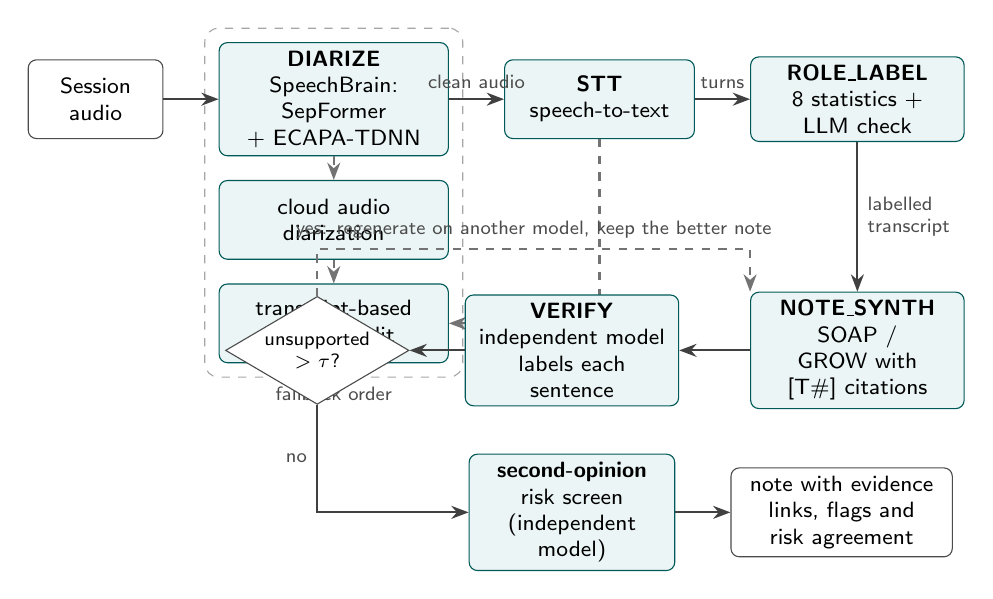
\begin{tikzpicture}[
  font=\sffamily\footnotesize,
  >={Stealth[length=2.2mm]},
  stage/.style={draw=black!70, rounded corners=3pt, fill=white, align=center, minimum height=10mm, inner sep=3pt, text width=#1},
  stage/.default=21mm,
  role/.style={draw=teal!70!black, rounded corners=3pt, fill=teal!8, align=center, minimum height=10mm, inner sep=3pt, text width=#1},
  role/.default=21mm,
  decision/.style={draw=black!70, diamond, aspect=1.7, fill=white, align=center, inner sep=1pt, font=\sffamily\scriptsize},
  flow/.style={->, thick, black!75},
  alt/.style={->, thick, dashed, black!55},
  lbl/.style={font=\sffamily\scriptsize, text=black!70},
  group/.style={draw=black!35, rounded corners=5pt, dashed, inner sep=5pt}
]
% ── row 1: audio → speaker separation → STT → roles ──
\node[stage=15mm] (audio) {Session\\audio};
\node[role=27mm, right=7mm of audio] (sb) {\textbf{DIARIZE}\\SpeechBrain: SepFormer\\+ ECAPA-TDNN};
\node[role=27mm, below=3mm of sb] (cloud) {cloud audio\\diarization};
\node[role=27mm, below=3mm of cloud] (text) {transcript-based\\speaker split};
\node[role=22mm, right=7mm of sb] (stt) {\textbf{STT}\\speech-to-text};
\node[role=25mm, right=7mm of stt] (roles) {\textbf{ROLE\_LABEL}\\8 statistics +\\LLM check};
\node[group, fit=(sb)(cloud)(text), label={[lbl]below:fallback order}] (diargrp) {};

\draw[flow] (audio) -- (sb);
\draw[alt] (sb) -- (cloud);
\draw[alt] (cloud) -- (text);
\draw[flow] (sb) -- node[lbl, above] {clean audio} (stt);
\draw[flow] (stt) -- node[lbl, above] {turns} (roles);
\draw[alt] (stt.south) |- (text.east);

% ── row 2: note writing, verification, gate, risk ──
\node[role=25mm, below=19mm of roles] (writer) {\textbf{NOTE\_SYNTH}\\SOAP / GROW with\\{[}T\#{]} citations};
\node[role=25mm, left=9mm of writer] (verify) {\textbf{VERIFY}\\independent model\\labels each sentence};
\node[decision, left=7mm of verify] (gate) {unsupported\\$>\tau$?};
\node[role=24mm, below=6mm of verify] (risk) {\textbf{second-opinion}\\risk screen\\(independent model)};
\node[stage=26mm, right=7mm of risk] (out) {note with evidence\\links, flags and\\risk agreement};

\draw[flow] (roles) -- node[lbl, right, align=left] {labelled\\transcript} (writer);
\draw[flow] (writer) -- (verify);
\draw[flow] (verify) -- (gate);
\draw[alt] (gate.north) -- ++(0,6mm) -| node[lbl, pos=0.25, above] {yes: regenerate on another model, keep the better note} (writer.north west);
\draw[flow] (gate.south) |- node[lbl, pos=0.25, left] {no} (risk.west);
\draw[flow] (risk) -- (out);
\end{tikzpicture}

\caption{EchoScribe pipeline. Shaded boxes are processing roles, each served by a combo of the embedded router (Section~\ref{sec:router}). Speaker separation falls back from local pyannote to cloud audio diarization to a transcript-based split (dashed). The note writer cites transcript turns; an independent model (another vendor, else another model) verifies each sentence, and notes over the unsupported threshold $\tau$ are regenerated on another model. A second model screens independently for risk.}
\label{fig:pipeline}
\end{figure*}

Fig.~\ref{fig:pipeline} shows the pipeline. A browser client records or uploads audio, an Express.js server coordinates every model call, and Supabase stores records under per-user row-level security. Five roles call language or speech models: \role{STT}, \role{DIARIZE}, \role{ROLE\_LABEL}, \role{NOTE\_SYNTH} and \role{VERIFY}.

\subsection{Embedded multi-provider router}\label{sec:router}
Each role is served by a \emph{combo}: an ordered list of targets $\langle$vendor, model, keys$\rangle$ and a routing strategy. Vendors are thin adapters: Gemini~\cite{gemini2023}, Groq-hosted gpt-oss-120b~\cite{openai2025gptoss} and Whisper~\cite{radford2023whisper}, Deepgram and a local pyannote service ship with the system. Several keys for one model form a pool whose keys take turns. The strategy orders targets per request: \emph{priority} (declared order; the next target is used only when every key of the current one is cooling down or retired, or the model itself fails), \emph{round-robin}, \emph{random}, \emph{strict-random}, \emph{least-used}, and \emph{lkgp} (the last target that succeeded goes first).

Failures are classified. A key that fails authentication is retired; a rate-limited or failing key enters an exponential cooldown of $5\cdot 2^{k-1}$~s (capped at 5~min) after its $k$-th consecutive failure, reset on success; a vendor with 15 failures within 30~min is skipped for 10~min (2 in 5~min for the local service); an HTTP~400 is treated as specific to the request and moves on without cooling the key.  Keys stay in the user's browser unless the user syncs one, which is then stored encrypted.

\subsection{Speech processing and role resolution}\label{sec:speech}
The recording is not denoised: SepFormer enhancement, our first design, raised word error rates (Section~\ref{sec:eval}), as reported for other front ends~\cite{iwamoto2022}. \role{DIARIZE} runs pyannote community-1~\cite{bredin2023pyannote,plaquet2023powerset} locally on the original 16~kHz recording, on a GPU when present, with two speakers and non-overlapping turns; it falls back to cloud audio diarization, then to splitting the transcript with a language model. \role{STT} transcribes the original recording; when the recogniser returns word timestamps (Whisper, Deepgram), each word goes to the turn that contains it~\cite{bain2023whisperx}, otherwise text is spread over turns by duration. 

Roles are resolved without voice enrolment. For each speaker the system computes eight statistics: speaking time, word count and mean turn length, questions, professional vocabulary, guiding phrases, personal and emotional phrases, number of turns, and who spoke first. \role{ROLE\_LABEL} receives the transcript with these statistics and must assign exactly one professional and one client; invalid answers move to the next target, and a deterministic default is used only if every target fails.

\subsection{Evidence-linked notes, verification and repair}\label{sec:grounding}
The labelled transcript is numbered into turns $T_1\dots T_n$. \role{NOTE\_SYNTH} must end every sentence of the note sections, and of the risk notes, with the turns that support it (``\dots poor sleep for two weeks [T4, T6]''), write one fact per sentence, and write ``Not discussed'' rather than an uncited sentence. \role{VERIFY} receives each sentence with only its cited turns and labels it \emph{supported}, \emph{partial} (adds a detail the turns lack) or \emph{unsupported}. Verifiers are ordered another vendor first, then another model of the writer's vendor, and never the writer's own model. If the unsupported fraction exceeds $\tau=0.2$, the note is regenerated with the writer's model moved to the end of the combo, re-verified, and the draft with fewer unsupported sentences is kept.

Two further steps work at sentence level. \emph{Repair}: each flagged sentence goes back to a writer model with the transcript and the verifier's reason to be rewritten with citations, or removed if the transcript does not support it; rewrites are verified again. \emph{Two-judge agreement}: a flag stands only if a second judge, chosen to differ from the first and from the writer, also flags it. \ifrecheck These steps are evaluated in Section~\ref{sec:eval}.\else They are implemented in the released code but not evaluated in this paper.\fi The interface shows each sentence's evidence on hover and marks partial and unsupported sentences (Fig.~\ref{fig:ui}); an \emph{Audio} button downloads the saved recording.

\begin{figure}[t]
\centering
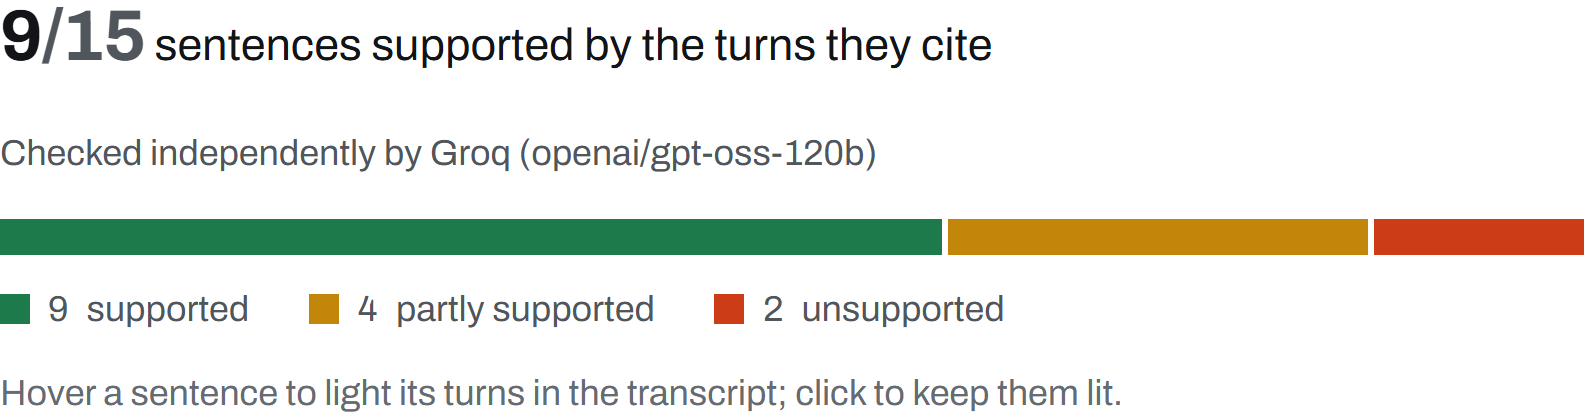
\includegraphics[width=0.56\columnwidth]{figures/ui_bar.png}\\[3pt]
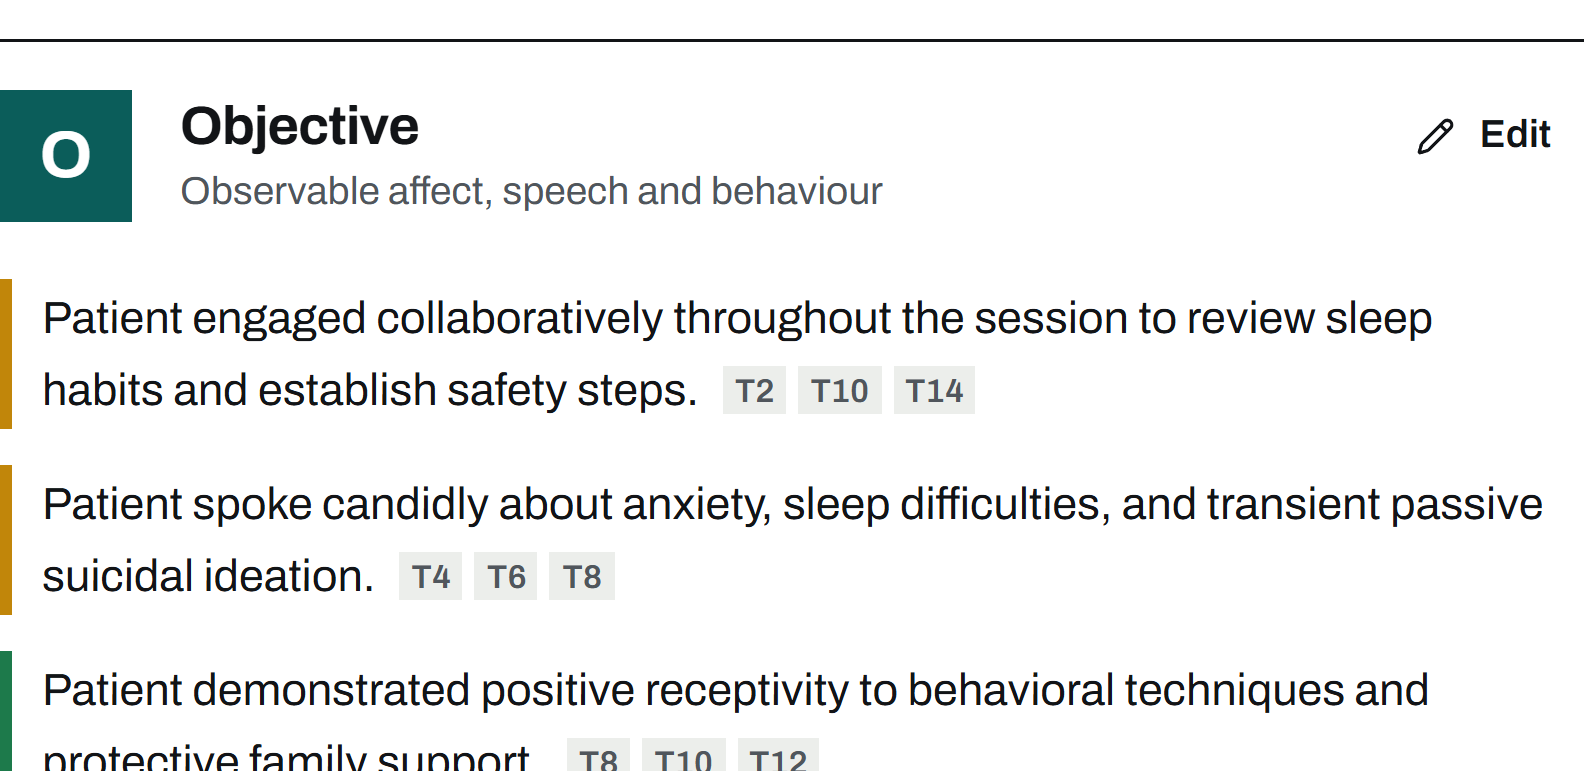
\includegraphics[width=0.56\columnwidth]{figures/ui_objective.png}
\caption{EchoScribe's session summary for a scripted example session (invented transcript; real pipeline output). The verification bar counts sentences the independent verifier (here gpt-oss-120b, checking a Gemini-written note) judged supported, partly supported or unsupported; Objective sentences carry a stripe for their label (green supported, amber partly, red unsupported) and the turns they cite.}
\label{fig:ui}
\end{figure}

\subsection{Risk screen with a second opinion}
In therapy mode the writer also screens for suicidal ideation and self-harm; in mentoring mode, for burnout and severe distress. A second model, chosen like the verifier, repeats the screen independently and cites its evidence turns. The flag is raised if either model raises it, favouring sensitivity, and disagreement is shown as ``models disagree --- review the transcript''. The screen is a model judgement, not a validated instrument such as the C-SSRS or PHQ-9~\cite{posner2011cssrs,kroenke2001phq9}, and the interface states that the clinician remains responsible for risk assessment.

\section{Evaluation}\label{sec:eval}
All experiments are scripted in the public repository (\texttt{eval/}) and every number below is generated from their result files.

\subsection{Setup}
\textbf{Data.} Note generation, verification and role identification use the 40 test dialogues of ACI-Bench (test1, CC~BY~4.0)~\cite{yim2023aci}, whose doctor--patient visits have reference notes; no public corpus of therapy or mentoring sessions with reference notes exists. Speech experiments use 12 simulated two-person conversations (12.5~min) built from LibriSpeech test-clean~\cite{panayotov2015librispeech}: ten alternating utterances from a mixed-gender speaker pair with 0.3--0.9~s gaps, exact reference turns, and three conditions, clean and with babble plus pink noise at 5~dB and 0~dB SNR.
\textbf{Models.} Gemini models~\cite{gemini2023} are used in rotation across three keys; gpt-oss-120b~\cite{openai2025gptoss} and Whisper large-v3~\cite{radford2023whisper} are served by Groq. The model that served each request is logged.
\textbf{Metrics.} ROUGE~\cite{lin2004rouge} and BERTScore~\cite{zhang2020bertscore} against reference notes; WER after text normalisation; DER with a 0.25~s collar~\cite{bredin2017metrics}; and cpWER, the speaker-attributed WER of CHiME-6~\cite{watanabe2020chime6}, which scores every speaker-separation path including those without timings. Intervals are Wilson 95\%.

\subsection{Router under injected faults}
We drive the router's own code with simulated vendors on a virtual clock: one hour of Poisson traffic at 10 requests/min against a preferred vendor (two keys), a fallback vendor (two keys) and a second fallback, in three scenarios: a per-key quota below the offered load (\emph{quota}); a 15-minute outage of the preferred vendor (\emph{outage}); and a revoked key, a quota and a fallback that times out 20\% of the time (\emph{mixed}). We compare walking the chain on every request with no memory, the fixed 60~s suspension of our earlier design, and the router with three strategies (5 seeds each, Table~\ref{tab:router}).

\begin{table}[t]
\caption{Router under injected faults (mean of 5 seeds): success rate, failed provider calls per request, and 95th-percentile latency (s).}
\label{tab:router}
\centering\footnotesize
\setlength{\tabcolsep}{3pt}
\begin{tabular}{@{}lrrrrrrrrr@{}}
\toprule
 & \multicolumn{3}{c}{Quota} & \multicolumn{3}{c}{Outage} & \multicolumn{3}{c}{Mixed} \\
\cmidrule(lr){2-4}\cmidrule(lr){5-7}\cmidrule(l){8-10}
Policy & Succ. & Fail & p95 & Succ. & Fail & p95 & Succ. & Fail & p95 \\
\midrule
No memory   & \ResRouterQuotaNomemorySuccess & \ResRouterQuotaNomemoryFailed & \ResRouterQuotaNomemoryPninetyfive & \ResRouterOutageNomemorySuccess & \ResRouterOutageNomemoryFailed & \ResRouterOutageNomemoryPninetyfive & \ResRouterMixedNomemorySuccess & \ResRouterMixedNomemoryFailed & \ResRouterMixedNomemoryPninetyfive \\
Fixed 60 s  & \ResRouterQuotaFixedSuccess & \ResRouterQuotaFixedFailed & \ResRouterQuotaFixedPninetyfive & \ResRouterOutageFixedSuccess & \ResRouterOutageFixedFailed & \ResRouterOutageFixedPninetyfive & \ResRouterMixedFixedSuccess & \ResRouterMixedFixedFailed & \ResRouterMixedFixedPninetyfive \\
Priority    & \ResRouterQuotaPrioritySuccess & \ResRouterQuotaPriorityFailed & \ResRouterQuotaPriorityPninetyfive & \ResRouterOutagePrioritySuccess & \ResRouterOutagePriorityFailed & \ResRouterOutagePriorityPninetyfive & \ResRouterMixedPrioritySuccess & \ResRouterMixedPriorityFailed & \ResRouterMixedPriorityPninetyfive \\
Round-robin & \ResRouterQuotaRoundrobinSuccess & \ResRouterQuotaRoundrobinFailed & \ResRouterQuotaRoundrobinPninetyfive & \ResRouterOutageRoundrobinSuccess & \ResRouterOutageRoundrobinFailed & \ResRouterOutageRoundrobinPninetyfive & \ResRouterMixedRoundrobinSuccess & \ResRouterMixedRoundrobinFailed & \ResRouterMixedRoundrobinPninetyfive \\
LKGP        & \ResRouterQuotaLkgpSuccess & \ResRouterQuotaLkgpFailed & \ResRouterQuotaLkgpPninetyfive & \ResRouterOutageLkgpSuccess & \ResRouterOutageLkgpFailed & \ResRouterOutageLkgpPninetyfive & \ResRouterMixedLkgpSuccess & \ResRouterMixedLkgpFailed & \ResRouterMixedLkgpPninetyfive \\
\bottomrule
\end{tabular}
\end{table}

No policy changes success much where a healthy fallback exists, so the differences lie in wasted calls and latency. The last-known-good strategy stops returning to a vendor that keeps timing out and reduces 95th-percentile latency in the mixed scenario from \ResRouterMixedPriorityPninetyfive~s to \ResRouterMixedLkgpPninetyfive~s; round-robin wastes the fewest calls and spreads load most evenly (Jain index~\cite{jain1984fairness} \ResRouterQuotaRoundrobinJain\ under quota pressure). Exponential cooldown alone is not uniformly better than a fixed suspension: under a persistent per-minute quota its 5~s first step re-probes an exhausted key (\ResRouterQuotaPriorityFailed\ against \ResRouterQuotaFixedFailed\ failed calls per request), while the fixed rule can suspend every option at once and lost requests in the mixed scenario (\ResRouterMixedFixedSuccess\ success). Priority keeps the clinician's preferred model at the cost of probing; LKGP minimises latency but can stay on a fallback model after the preferred one recovers.

\subsection{Evidence-linked notes and independent verification}
Each of the two writers produced a SOAP note with turn citations for the 40 test dialogues, and a model other than the writer verified every sentence (Table~\ref{tab:notes}). Because the Groq free tier's daily token cap was reached during the runs, verification of Gemini-written notes was cross-vendor for \ResVerGemCrossVendor\ notes and cross-model (another Gemini model) for \ResVerGemCrossModel; for gpt-oss-written notes it was cross-vendor for \ResVerGroqCrossVendor\ and cross-model for \ResVerGroqCrossModel. Notes the writer's own model had checked during a quota fallback (\ResVerGemExcluded\ and \ResVerGroqExcluded\ after re-verification) are excluded from the support figures. Citation coverage was \ResGroundGemCited\ (Gemini) and \ResGroundGroqCited\ (gpt-oss-120b); \ResGroundGemSupported\ and \ResGroundGroqSupported\ of sentences were judged fully supported and \ResGroundGemUnsupported\ and \ResGroundGroqUnsupported\ unsupported. With the gate at $\tau=0.2$, \ResCascadeEscalated\ of \ResCascadeNotes\ Gemini-first notes would have been regenerated. ROUGE against ACI-Bench reference notes measures overlap with a differently structured visit note and is reported for comparability, not as a quality ceiling.

\begin{table}[t]
\caption{Notes on ACI-Bench test1: overlap with reference notes and independent verification of every sentence.}
\label{tab:notes}
\centering\footnotesize
\setlength{\tabcolsep}{4pt}
\begin{tabular}{@{}lrr@{}}
\toprule
Writer (verifier) & Gemini (gpt-oss) & gpt-oss (Gemini) \\
\midrule
Notes & \ResNoteGemN & \ResNoteGroqN \\
ROUGE-1 / 2 / L & \ResNoteGemRougeOne\,/\,\ResNoteGemRougeTwo\,/\,\ResNoteGemRougeL & \ResNoteGroqRougeOne\,/\,\ResNoteGroqRougeTwo\,/\,\ResNoteGroqRougeL \\
BERTScore F1 & \ResNoteGemBert & \ResNoteGroqBert \\
Sentences per note & \ResGroundGemSentences & \ResGroundGroqSentences \\
Sentences with citations & \ResGroundGemCited & \ResGroundGroqCited \\
Supported / partial & \ResGroundGemSupported\,/\,\ResGroundGemPartial & \ResGroundGroqSupported\,/\,\ResGroundGroqPartial \\
Unsupported & \ResGroundGemUnsupported & \ResGroundGroqUnsupported \\
Notes over gate ($\tau$=0.2) & \ResGroundGemOverGate & \ResGroundGroqOverGate \\
\midrule
Planted errors caught: number & \ResInjGemNum & \ResInjGroqNum \\
\quad negation & \ResInjGemNeg & \ResInjGroqNeg \\
\quad borrowed sentence & \ResInjGemFab & \ResInjGroqFab \\
False alarms on unchanged & \ResInjGemFa & \ResInjGroqFa \\
\bottomrule
\end{tabular}
\end{table}

\textbf{Does the verifier catch errors?} Model-judged support is only useful if the judge detects real errors. We planted three kinds of error into sentences the verifier had accepted: a changed number, a flipped negation, and a sentence borrowed from another dialogue's note with the original citations; other accepted sentences were kept as controls. Across \ResInjPlantedN\ planted errors the verifier flagged \ResInjRecallPct\ as partial or unsupported, with \ResInjFaPct\ false alarms on \ResInjControlN\ unchanged sentences (Table~\ref{tab:notes}, bottom). Controls were sentences this verifier had already accepted, so the false-alarm rate measures consistency rather than precision on fresh sentences.

\subsection{Role identification}
With doctor and patient labels replaced by random speaker identifiers, the eight statistics alone named the clinician correctly in \ResRoleStatsCorrect\ of \ResRoleN\ dialogues (\ResRoleStats), the model alone in \ResRoleLlmCorrect\ (\ResRoleLlm), and their combination, as deployed, in \ResRoleCombinedCorrect\ (\ResRoleCombined). Only \ResRoleHardN\ dialogues had the patient speaking more than the doctor, too few to test the case the statistics are meant for; this is part of the role-play protocol below.

\subsection{Speech recognition and speaker attribution}
\begin{table}[t]
\caption{Simulated two-person conversations (12 $\times$ 3 conditions): WER of speech-to-text with and without SepFormer, DER of SpeechBrain clustering, and speaker-attributed cpWER of each separation path (\%).}
\label{tab:speech}
\centering\footnotesize
\setlength{\tabcolsep}{4pt}
\begin{tabular}{@{}lrrr@{}}
\toprule
 & Clean & 5 dB & 0 dB \\
\midrule
WER Gemini, raw / enhanced & \ResAudioWerGemRawClean\,/\,\ResAudioWerGemEnhClean & \ResAudioWerGemRawFive\,/\,\ResAudioWerGemEnhFive & \ResAudioWerGemRawZero\,/\,\ResAudioWerGemEnhZero \\
WER Whisper, raw / enhanced & \ResAudioWerGroqRawClean\,/\,\ResAudioWerGroqEnhClean & \ResAudioWerGroqRawFive\,/\,\ResAudioWerGroqEnhFive & \ResAudioWerGroqRawZero\,/\,\ResAudioWerGroqEnhZero \\
DER SpeechBrain, raw / enh. & \ResAudioDerSbRawClean\,/\,\ResAudioDerSbEnhClean & \ResAudioDerSbRawFive\,/\,\ResAudioDerSbEnhFive & \ResAudioDerSbRawZero\,/\,\ResAudioDerSbEnhZero \\
\midrule
cpWER SpeechBrain + STT & \ResAudioCpSbRawClean & \ResAudioCpSbRawFive & \ResAudioCpSbRawZero \\
cpWER cloud audio diarization & \ResAudioCpGemAudioClean & \ResAudioCpGemAudioFive & \ResAudioCpGemAudioZero \\
cpWER transcript-based split & \ResAudioCpTextClean & \ResAudioCpTextFive & \ResAudioCpTextZero \\
\bottomrule
\end{tabular}
\end{table}

Table~\ref{tab:speech} reports the speech results. Denoising before recognition, as in our first design, raised word error rates under noise for both recognisers (for Whisper at 0~dB from \ResAudioWerGroqRawZero\% to \ResAudioWerGroqEnhZero\%), so the deployed pipeline transcribes the original recording. pyannote separated speakers with \ResAudioDerPyaClean\% DER on clean audio against \ResAudioDerSbRawClean\% for SpeechBrain clustering. Speaker attribution depends as much on placing words as on finding turns: spreading the transcript over pyannote's turns by duration gave \ResAudioCpPyaPropClean\% cpWER, assigning each word to the turn containing its Whisper timestamp gave \ResAudioCpPyaWordsClean\%, and at 5~dB \ResAudioCpPyaWordsFive\% against \ResAudioCpGemAudioFive\% for cloud audio diarization. At 0~dB pyannote's DER rises to \ResAudioDerPyaZero\% and SpeechBrain clustering with word timestamps attributes slightly better (\ResAudioCpSbWordsZero\% against \ResAudioCpPyaWordsZero\%).


Processing cost per minute of audio on a laptop CPU was \ResLatSbEnh~s for SepFormer enhancement with diarization (windowed, bounded memory), \ResLatSbDiar~s for diarization alone, \ResLatSttGroq~s for Whisper on Groq and \ResLatSttGem~s for Gemini speech-to-text.


\section{Discussion and Limitations}
\textbf{What the results support.} Citation-constrained writing halved unsupported content against a single-pass note without lowering overlap with reference notes, and an independent verifier caught most planted factual errors, so sentence-level flags give a reviewer a concrete place to look instead of an unexplained confidence score~\cite{guo2017calibration}. Resilience in the router comes from remembering failures. Placing words by timestamp, not turn duration, accounts for most of the gain in speaker attribution on simulated and acted speech, and role identification without enrolment was accurate on medical and counselling dialogue.

\textbf{Deployment.} EchoScribe runs on the clinician's machine; only the configured model vendors receive audio or text, an institution can restrict processing to vendors its governance policy approves, and long recordings are compacted before reaching a cloud model.

\textbf{Limitations.} (i) ACI-Bench and PriMock57 are medical, and AnnoMI has no reference notes; no public corpus of counselling or mentoring sessions with reference notes exists\ifmentoring, and the mentoring sessions we ran are few and not independent\else, so GROW notes were not evaluated\fi. (ii) Support labels come from a model; the planted-error test bounds how often it misses errors of three kinds, but subtler omissions and misattributions need human review~\cite{asgari2025}, and where a quota forced a judge from the writer's vendor the check was not vendor-independent. (iii) Simulated speech is read without overlap, and PriMock57 is acted speech; overlapping, emotional clinical speech will be harder, and at 0~dB our attribution is not better than cloud diarization. (iv) Results depend on specific model versions that vendors retire; we log the serving model of every request. (v) The risk screen has not been validated against clinician labels. Blinded rating kits for notes and verifier agreement are released with the code. \textbf{Ethics:} no human-subject data were used; all experiments use public datasets and scripted or synthetic material, and free-tier model vendors may use submitted text for training, so deployments with real sessions should use institutionally approved vendors or local models.


\section{Conclusion}
EchoScribe produces SOAP and GROW notes from recorded two-person sessions in which every sentence points to the turns that support it and is checked by a model from a different vendor, with a verification-gated cascade, a two-model risk screen that surfaces disagreement, and an embedded router that keeps every processing role available through quota exhaustion, outages and revoked keys. On public data the notes were almost fully cited, the cross-vendor verifier caught most planted errors, role identification needed no enrolment, and the router's last-known-good strategy cut tail latency under compound faults. The code, evaluation scripts and human-evaluation protocol are available at \url{https://github.com/Aravind-Krishnan-S/ECHOSCRIBE}.


\section*{Acknowledgment}
The authors thank the faculty of the Department of Artificial Intelligence and Data Science at Jyothi Engineering College for their guidance, and the pyannote, SpeechBrain, ACI-Bench, AnnoMI, PriMock57, LibriSpeech and OmniRoute communities for openly licensed models, data and code. Claude (Anthropic) was used to draft and revise the manuscript text and LaTeX, and to write parts of the software and evaluation code; the authors directed, verified and take responsibility for all content.

\bibliographystyle{IEEEtran}
\bibliography{refs}

\end{document}
